% --- FILE: 4.3_rag_pipeline/4.3.0_intro.tex ---

\section{Mô hình Truy xuất và Tạo sinh tri thức (RAG Module)}
\label{sec:rag_pipeline}

Tiếp nối kết quả từ quá trình chuyển đổi giọng nói sang văn bản, mô-đun \gls{rag} đóng vai trò trung tâm trong việc tổ chức, khai thác và tổng hợp tri thức từ dữ liệu hội thoại. Dựa trên đầu vào là các tệp JSON có cấu trúc (chứa thông tin người nói, thời gian và nội dung) từ mô-đun ASR, mô-đun này được thiết kế để thực hiện hai nhóm chức năng cốt lõi:\textit{Truy xuất thông tin theo ngữ cảnh} (phục vụ hỏi đáp) và \textit{Tổng hợp nội dung đa tầng}(phục vụ tóm tắt).

Để hiện thực hóa các chức năng trên, mô-đun vận hành theo một quy trình xử lý khép kín gồm bốn giai đoạn kỹ thuật chính:

\begin{enumerate}
    \item \textbf{Indexing (Đánh chỉ mục):} Mã hóa văn bản thành vector và lưu trữ vào cơ sở dữ liệu chuyên dụng, kèm theo siêu dữ liệu để phục vụ lọc thông tin.
    \item \textbf{Retrieval (Truy xuất):} Tìm kiếm các đoạn hội thoại liên quan nhất đến câu hỏi dựa trên ngữ nghĩa (Semantic Search) và xếp hạng lại (Re-ranking) để loại bỏ nhiễu.
    \item \textbf{Generation (Tạo sinh):} Tích hợp \gls{llm} để sinh câu trả lời tự nhiên hoặc bản tóm tắt dựa trên ngữ cảnh đã trích xuất.
    \item \textbf{Summarization (Tổng hợp):} Áp dụng các kỹ thuật xử lý ngữ cảnh dài để tóm tắt toàn bộ cuộc họp hoặc tóm tắt theo từng đối tượng người nói cụ thể.
\end{enumerate}



\begin{figure}[H]
    \centering
    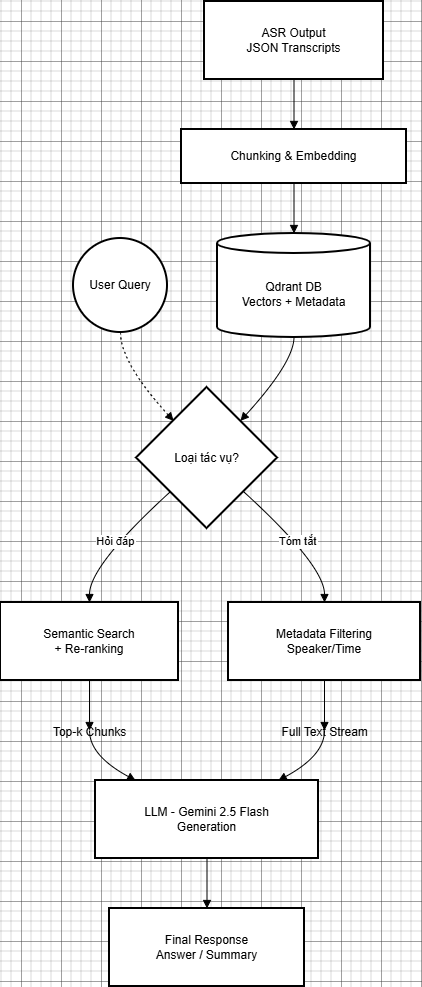
\includegraphics[width=0.6\textwidth]{images/RAG_pipline.png}
    \caption{Sơ đồ luồng xử lý dữ liệu tích hợp chức năng Tóm tắt trong mô-đun RAG}
    \label{fig:rag_detailed_flow}
\end{figure}
\clearpage